% =====================================================================
%  CV — Elliott Sainte-Catherine
%  Compilation : pdflatex CV_SainteCatherine_Elliott.tex
%  (nécessite les packages : geometry, paracol, enumitem, titlesec,
%   xcolor, hyperref, fontawesome5, graphicx — tous inclus dans TeX Live)
% =====================================================================
\documentclass[10pt,a4paper]{article}

\usepackage[utf8]{inputenc}
\usepackage[T1]{fontenc}
\usepackage[french]{babel}
\usepackage[a4paper,margin=1.2cm,top=1cm,bottom=1cm]{geometry}
\usepackage{graphicx}
\usepackage{paracol}
\usepackage{enumitem}
\usepackage{titlesec}
\usepackage{xcolor}
\usepackage{fontawesome5}
\usepackage[hidelinks]{hyperref}
\usepackage{helvet}
\renewcommand{\familydefault}{\sfdefault}

\definecolor{darkgray}{HTML}{2B2B2B}
\color{darkgray}

\pagestyle{empty}
\setlength{\parindent}{0pt}

% ------- styles de sections -------
\titleformat{\section}{\Large\bfseries}{}{0pt}{}
\titlespacing*{\section}{0pt}{8pt}{4pt}
\titleformat{\subsection}{\large\bfseries}{}{0pt}{}
\titlespacing*{\subsection}{0pt}{6pt}{2pt}

\newcommand{\datetag}[1]{\hfill{\small\bfseries #1}}
\setlist[itemize]{leftmargin=*,nosep,itemsep=2pt,label=\textbullet}

\begin{document}

% =====================  EN-TÊTE  =====================
\begin{minipage}[c]{0.22\textwidth}
    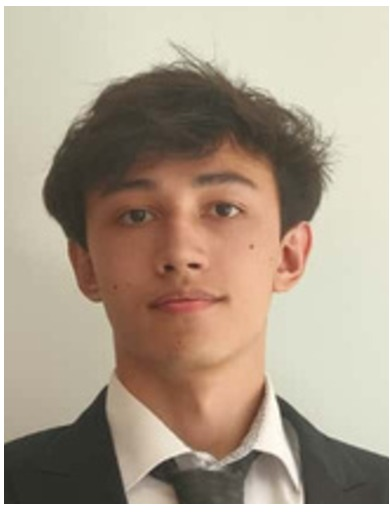
\includegraphics[width=\linewidth]{photo.jpg}
\end{minipage}\hfill
\begin{minipage}[c]{0.75\textwidth}
    \centering
    {\Large\bfseries STAGE INGÉNIEUR SPATIAL (FIN D'ÉTUDES)}\\[2pt]
    {\large 6 mois à partir de février 2026 -- Ingénierie Système \& Propulsion}\\[8pt]
    {\LARGE\bfseries E L L I O T T\ \ S A I N T E - C A T H E R I N E}\\[8pt]
    \faPhone\ +33 7 82 64 55 35 \quad
    \faEnvelope\ \href{mailto:elliott.sainte-catherine@epfedu.fr}{elliott.sainte-catherine@epfedu.fr}\\[3pt]
    \faLinkedin\ \href{https://www.linkedin.com/}{Elliott Sainte-Catherine} \quad
    \faMapMarker*\ 92400 Courbevoie
\end{minipage}

\vspace{4pt}
\hrule height 1pt
\vspace{6pt}

% =====================  DEUX COLONNES  =====================
\columnratio{0.31}
\setlength{\columnsep}{16pt}
\begin{paracol}{2}

% --------------------- COLONNE GAUCHE ---------------------
\raggedright
\emergencystretch=1.5em
\section{PROFIL}
Futur ingénieur aérospatial spécialisé en propulsion et systèmes.
Fort d'une expérience pratique en conception de fusées (association)
et en ingénierie système, je cherche à contribuer au développement
de lanceurs innovants.

\section{COMPÉTENCES}
\begin{itemize}
    \item Programmation : Java, Python, C++, SQL, VBA, Excel, Matlab (Simulink)
    \item Utilisation de Git et GitHub
    \item Modélisation : CATIA, COMSOL, Amesim, Ansys (FLUENT)
    \item Impression 3D : Orca Slicer
    \item Machine learning
    \item Analyse critique
    \item Travail d'équipe
    \item Prise d'initiative
\end{itemize}

\section{LANGUES}
{\itshape Expatrié à Singapour de 2006 à 2010}
\begin{itemize}
    \item Français courant
    \item Anglais 950 TOEIC (C1)
    \item Mandarin (langue maternelle -- oral)
\end{itemize}

\section{HOBBIES}
\begin{itemize}
    \item Piano (11 ans et spectacles)
    \item Team gym (Championnat de France)
    \item Triathlon
    \item Dessin
\end{itemize}

% --------------------- COLONNE DROITE ---------------------
\switchcolumn

\section{ENSEIGNEMENTS ACADÉMIQUES}
\subsection{Cursus ingénieur généraliste \datetag{2021--2026}}
\textbf{EPF ENGINEERING SCHOOL (Cachan)}\\
5\ieme{} année du cycle ingénieur, majeure aéronautique et espace

\vspace{2pt}
\begin{minipage}[t]{0.46\linewidth}
    \begin{itemize}
        \item Ingénierie système
        \item Propulsion Spatiale
        \item Mécanique des fluides
    \end{itemize}
\end{minipage}\hfill
\begin{minipage}[t]{0.5\linewidth}
    \begin{itemize}
        \item Fatigue--Tolérance aux dommages
        \item Méthodes Statistiques pour l'Ingénieur
        \item Aérodynamique (CFD)
    \end{itemize}
\end{minipage}

\vspace{4pt}
\hrule
\vspace{4pt}

\section{EXPÉRIENCES}

\begin{minipage}[t]{0.53\linewidth}
    \subsection{EPF ASTRONOMIE \datetag{2023--2026\ \ 3 ans}}
    Vice-président, trésorier, chef de projet minifusée et de propulsion solide
    \begin{itemize}
        \item Conception et lancement de fusées expérimentales au C'Space
        \item Dimensionnement et préparation de la campagne de tir statique
              (moteur solide)
        \item Analyses mécaniques (structure) et thermodynamiques
              (performances) associées
        \item Pilotage de deux équipes (15 membres) : fusée et propulsion
        \item Pilotage du budget global et gestion des achats techniques
    \end{itemize}

    \subsection{Enseignant EPF \datetag{2025\ \ 2 mois}}
    Enseignant Chargé de Travaux Pratiques (TP) en fabrication additive
    \begin{itemize}
        \item Préparation des cours
        \item Formation d'étudiants en études supérieures
    \end{itemize}
\end{minipage}\hfill
\begin{minipage}[t]{0.43\linewidth}
    \subsection{Preconception d'un lanceur en partenariat avec le CNES}
    Projet d'école \datetag{2025\ \ 4 mois}
    \begin{itemize}
        \item Dimensionnement et analyse de stabilité des ergols (sloshing)
              et excitations d'un lanceur à 3 étages
        \item Performances moteur (NASA CEA) et calculs
        \item Calcul de trajectoire sur Lotus
    \end{itemize}

    \subsection{Estimation de la durée de vie de l'avion COMET}
    Projet d'école \datetag{2025\ \ 4 mois}
    \begin{itemize}
        \item Utilisation de modèles (Basquin, Whöler\ldots) et de critères
              (Crossland) pour dimensionner le hublot d'un avion COMET
              sur Matlab
    \end{itemize}
\end{minipage}

\vspace{4pt}
\hrule
\vspace{4pt}

\section{STAGES}

\subsection{Charlie-Fox Aviation Budapest \datetag{2024\ \ 4 mois\ \ {\normalfont\itshape(Stage élève ingénieur)}}}
Développement d'un simulateur de vol d'A320 AR/XR certifié FNPTII en
Bureau d'études
\begin{itemize}
    \item Élaboration d'un sidestick à partir des spécifications FNPTII EASA
    \item Assemblage et outillage (outils de chantier)
    \item Ingénierie système, spécification MOA, analyse fonctionnelle,
          étude de l'état de l'art, choix d'architecture et modélisation CAO
\end{itemize}

\subsection{POK SAS \datetag{2022\ \ 2 mois\ \ {\normalfont\itshape(Stage d'exécution)}}}
Ouvrier :
\begin{itemize}
    \item Analyse de plans d'assemblage, assemblage d'agrès incendie en
          chaîne de production et test de lances à incendie
\end{itemize}

\end{paracol}

\end{document}
